\section{Scientific Paper}

\begin{flushleft}
    This section presents the paper co-authored with my professor for the 24th International Conference on Agents and Multi-Agent Systems \href{https://aamas2025.org/}{(AAMAS 2025)}. It summarizes the key aspects of my research, including the problem definition, proposed methodology, and experimental results. It serves as a concise overview of my thesis, providing a snapshot of the research from a technical perspective.\\~\\

    The paper is included below in its original form to reflect the work as it was submitted.
\end{flushleft}

\newpage

\phantomsection
\addcontentsline{toc}{subsection}{1\hspace{1.8em}Introduction}
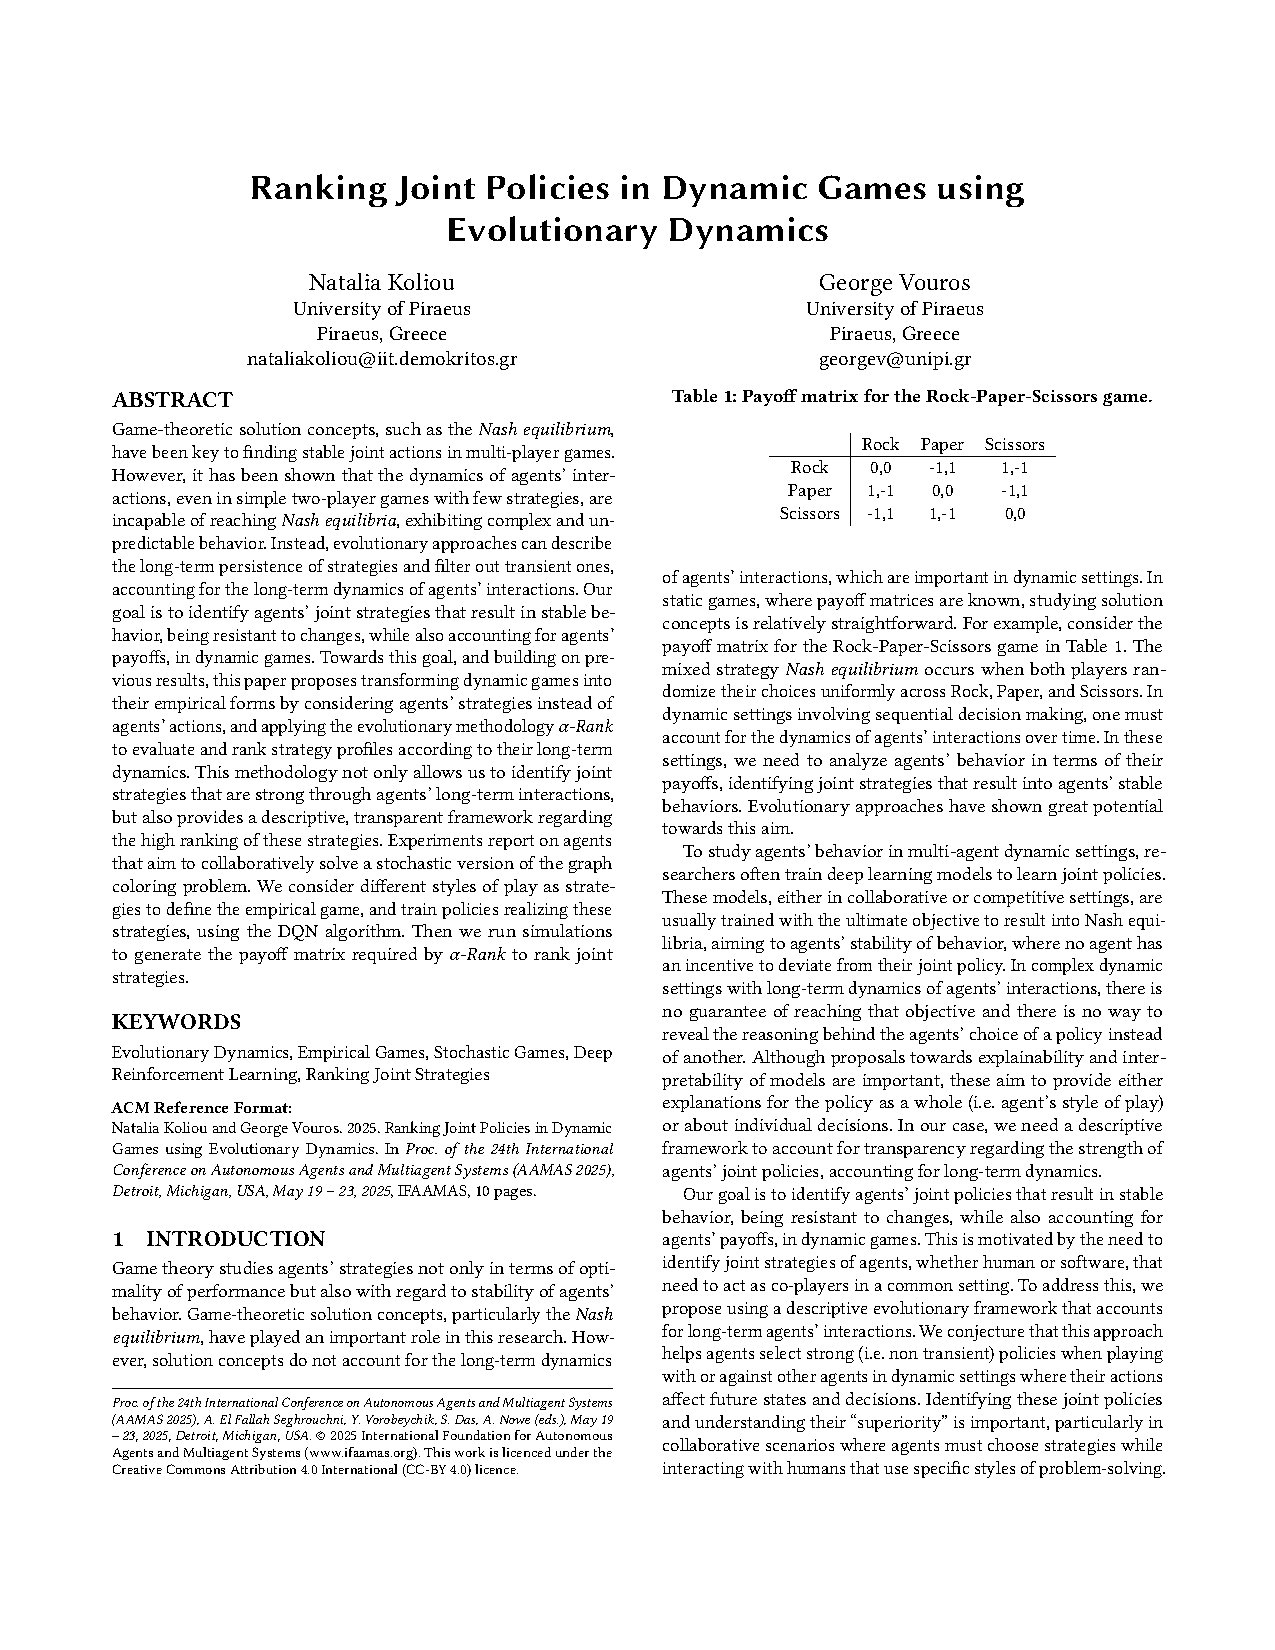
\includepdf[pages=1]{./paper.pdf}

\phantomsection
\addcontentsline{toc}{subsection}{2\hspace{1.8em}Background}

\phantomsection
\addcontentsline{toc}{subsubsection}{2.1\hspace{1.8em}Dynamic Games}

\phantomsection
\addcontentsline{toc}{subsubsection}{2.2\hspace{1.8em}Empirical Analysis and Empirical Games}

\includepdf[pages=2]{./paper.pdf}

\phantomsection
\addcontentsline{toc}{subsubsection}{2.3\hspace{1.8em}\texorpdfstring{The α-Rank Method}{}}

\includepdf[pages=3]{./paper.pdf}

\phantomsection
\addcontentsline{toc}{subsection}{3\hspace{1.8em}Problem Statement}

\phantomsection
\addcontentsline{toc}{subsection}{4\hspace{1.8em}Proposed Method}

\includepdf[pages=4]{./paper.pdf}

\phantomsection
\addcontentsline{toc}{subsection}{5\hspace{1.8em}Experiments and Results}

\phantomsection
\addcontentsline{toc}{subsubsection}{5.1\hspace{1.8em}The Graph Coloring Problem}

\phantomsection
\addcontentsline{toc}{subsubsection}{5.2\hspace{1.8em}Defining the Empirical Game}

\includepdf[pages=5]{./paper.pdf}

\phantomsection
\addcontentsline{toc}{subsubsection}{5.3\hspace{1.8em}Evaluation and Ranking}

\includepdf[pages=6-7]{./paper.pdf}

\phantomsection
\addcontentsline{toc}{subsection}{6\hspace{1.8em}Conclusions}

\includepdf[pages=8]{./paper.pdf}

\phantomsection
\addcontentsline{toc}{subsection}{Appendices}

\phantomsection
\addcontentsline{toc}{subsubsection}{A\hspace{1.8em}Empirical Payoff Matrix}

\includepdf[pages=9]{./paper.pdf}

\phantomsection
\addcontentsline{toc}{subsubsection}{B\hspace{1.8em}Response Graph}

\includepdf[pages=10]{./paper.pdf}